% ------------------------------------------------------------------------
% ------------------------------------------------------------------------
% D1INT - Atividade 2: Metodologias de gerenciamento de projetos de
% Ciência de Dados
% ------------------------------------------------------------------------
% ------------------------------------------------------------------------

\documentclass[
	% -- opções da classe memoir --
	article,			% indica que é um artigo acadêmico
	11pt,				% tamanho da fonte
	oneside,			% para impressão apenas no recto. Oposto a twoside
	a4paper,			% tamanho do papel.
	% -- opções da classe abntex2 --
	%chapter=TITLE,		% títulos de capítulos convertidos em letras maiúsculas
	%section=TITLE,		% títulos de seções convertidos em letras maiúsculas
	%subsection=TITLE,	% títulos de subseções convertidos em letras maiúsculas
	%subsubsection=TITLE % títulos de subsubseções convertidos em letras maiúsculas
	% -- opções do pacote babel --
	english,			% idioma adicional para hifenização
	brazil,				% o último idioma é o principal do documento
	sumario=tradicional
	]{abntex2}


% ---
% PACOTES
% ---

% ---
% Pacotes fundamentais
% ---
\usepackage{lmodern}			% Usa a fonte Latin Modern
\usepackage[T1]{fontenc}		% Selecao de codigos de fonte.
\usepackage[utf8]{inputenc}		% Codificacao do documento (conversão automática dos acentos)
\usepackage{indentfirst}		% Indenta o primeiro parágrafo de cada seção.
\usepackage{nomencl} 			% Lista de simbolos
\usepackage{color}				% Controle das cores
\usepackage{graphicx}			% Inclusão de gráficos
\usepackage{microtype} 			% para melhorias de justificação
% ---

% ---
% Pacotes adicionais, usados apenas no âmbito do Modelo Canônico do abnteX2
% ---
%\usepackage{lipsum}				% para geração de dummy text
% ---

% ---
% Pacotes de citações
% ---
\usepackage[brazilian,hyperpageref]{backref}	 % Paginas com as citações na bibl
\usepackage[alf]{abntex2cite}	% Citações padrão ABNT
% ---

% ---
% Configurações do pacote backref
% Usado sem a opção hyperpageref de backref
\renewcommand{\backrefpagesname}{Citado na(s) página(s):~}
% Texto padrão antes do número das páginas
\renewcommand{\backref}{}
% Define os textos da citação
\renewcommand*{\backrefalt}[4]{
	\ifcase #1 %
		Nenhuma citação no texto.%
	\or
		Citado na página #2.%
	\else
		Citado #1 vezes nas páginas #2.%
	\fi}%
% ---

% --- Informações de dados para CAPA e FOLHA DE ROSTO ---
\titulo{Metodologias de Gerenciamento de Projetos de Ciência de Dados}
%\tituloestrangeiro{Data Science Project Management Methodology}

\autor{
Diego Machado de Assis\thanks{
  CP301343X
  \href{mailto:diego.assis@aluno.ifsp.edu.br}{diego.assis@aluno.ifsp.edu.br}
}
}

\local{Brasil}
\data{15 de maio de 2021}
% ---

% ---
% Configurações de aparência do PDF final

% alterando o aspecto da cor azul
\definecolor{blue}{RGB}{41,5,195}

% informações do PDF
\makeatletter
\hypersetup{
     	%pagebackref=true,
		pdftitle={\@title},
		pdfauthor={\@author},
    	pdfsubject={Metodologias de Gerenciamento de Projetos em Ciência de Dados},
	    pdfcreator={Diego Machado de Assis},
		pdfkeywords={gerenciamento de projeto}{ciência de dados}{dados},
		colorlinks=true,       		% false: boxed links; true: colored links
    	linkcolor=blue,          	% color of internal links
    	citecolor=blue,        		% color of links to bibliography
    	filecolor=magenta,      		% color of file links
		urlcolor=blue,
		bookmarksdepth=4
}
\makeatother
% ---

% ---
% compila o indice
% ---
\makeindex
% ---

% ---
% Altera as margens padrões
% ---
\setlrmarginsandblock{3cm}{3cm}{*}
\setulmarginsandblock{3cm}{3cm}{*}
\checkandfixthelayout
% ---

% ---
% Espaçamentos entre linhas e parágrafos
% ---

% O tamanho do parágrafo é dado por:
\setlength{\parindent}{1.3cm}

% Controle do espaçamento entre um parágrafo e outro:
\setlength{\parskip}{0.2cm}  % tente também \onelineskip

% Espaçamento simples
\SingleSpacing


% ----
% Início do documento
% ----
\begin{document}

% Seleciona o idioma do documento (conforme pacotes do babel)
%\selectlanguage{english}
\selectlanguage{brazil}

% Retira espaço extra obsoleto entre as frases.
\frenchspacing

% ----------------------------------------------------------
% ELEMENTOS PRÉ-TEXTUAIS
% ----------------------------------------------------------

%---
%
% Se desejar escrever o artigo em duas colunas, descomente a linha abaixo
% e a linha com o texto ``FIM DE ARTIGO EM DUAS COLUNAS''.
% \twocolumn[    		% INICIO DE ARTIGO EM DUAS COLUNAS
%
%---

% página de titulo principal (obrigatório)
\maketitle


% titulo em outro idioma (opcional)



% resumo em português
\begin{resumoumacoluna}
 Metodologias de gerenciamento de projetos de Ciência de Dados podem ser grande
 aliadas no desenvolvimento de projetos robustos, eficazes e eficientes na área.
 Diversos padrões existem e atendem a uma grande heterogeneidade de necessidades
 e requisitos. Alguns destes padrões são mais amplamente utilizados e
 consolidados, tornando-se padrões \textit{de facto} na indústria. Este trabalho
 apresenta um breve resumo e traça um paralelo entre três das principais
 metodologias existentes hoje: \textit{KDD}, \textit{CRISP-DM} e \textit{SEMMA}.

 \vspace{\onelineskip}

 \noindent
 \textbf{Palavras-chave}: Ciência de dados. Gerenciamento de projetos. Mineração
 de dados. KDD. CRISP-DM. SEMMA.
\end{resumoumacoluna}

\begin{center}\smaller
\textbf{Data de submissão}: 06 de junho de 2021

\end{center}

% ----------------------------------------------------------
% ELEMENTOS TEXTUAIS
% ----------------------------------------------------------
\textual

% ----------------------------------------------------------
% Introdução
% ----------------------------------------------------------
\section{Introdução}

Métodos sistemáticos para extração de conhecimento a partir de dados ajudam a
organizar de forma estruturada o desenvolvimento e avaliação de respostas para
problemas de análise de dados \cite{provost2013}. Conhecer as principais
técnicas e etapas em um projeto de Ciência de Dados é fundamental para maior
acurácia dos resultados, ao mesmo tempo que o desenvolvimento seja o mais
eficiente e ágil possível.

Cada projeto possui suas particularidades e não existe metodologia ubíqua que
abstraia por completo as necessidades concretas de cada caso. Dessa forma,
conhecer os principais métodos e ferramentas disponíveis é fundamental para
composição do arsenal de um cientista de dados. Mais importante do que ranquear
os processos é conseguir entender as semelhanças e diferenças entre eles, assim
como identificar que tipo de problemas cada um se propõe a atacar.

Neste trabalho procuramos definir algumas das metodologias mais utilizadas hoje
e traçar um breve comparativo entre elas. Na seção \ref{sec:metodologias}
apresentamos as metodologias \textit{KDD}, \textit{CRISP-DM} e \textit{SEMMA}.
Na seção \ref{sec:diferencas} fazemos um paralelo entre as principais diferenças
entre elas e na seção \ref{sec:final} tentamos consolidar as ideias apresentadas
de cada uma e olhar qual nos seria mais adequada em um projeto de Ciência de
Dados.

% ----------------------------------------------------------
% Detalhamento das Metodologias
% ----------------------------------------------------------
\section{Metodologias de Gerenciamento de Projetos}
\label{sec:metodologias}

\subsection{KDD}

O processo de Extrair de Conhecimento a partir de Dados (ou
\textit{Knowledge Discovery from Data - KDD}) muitas vezes se confunde com o
próprio conceito de Mineração de Dados (ou \textit{Data Mining}). O processo de
KDD consiste em uma sequência iterativa das seguintes etapas \cite{han2006}:

\begin{enumerate}
  \item Limpeza dos dados
  \item Integração dos dados
  \item Seleção dos dados
  \item Transformação dos dados
  \item Mineração dos dados
  \item Avaliação dos padrões
  \item Apresentação dos resultados
\end{enumerate}

A \textbf{Limpeza dos dados} consiste na remoção de ruídos e dados
inconsistentes (\textit{outliers}). Nesta fase deve ser definida a estratégia
para tratamento de dados faltantes, assim como é feito o mapeamento dos
atributos com os seus respectivos tipos.

A \textbf{Integração dos dados} consiste na combinação de mútlipas fontes de
dados em um formato de armazenamento coerente e o salvamento dos mesmos em uma
fonte de fácil acesso (por exemplo um \textit{data warehouse}).

Na etapa de \textbf{Seleção de dados}, é realizada a seleção apenas dos dados
relevantes para os objetivos de análise pretendidos.

A \textbf{Transformação dos dados} objetiva consolidar os dados em um formato
apropriado para a etapa de mineração. Para tanto, podem ser realizadas
sumarizações, agregações, generalizações e normalizações do conjuto de dados.
Em alguns casos, esta etapa pode vir acompanhada de \textbf{Redução dos dados},
para que se tenha uma representação mais suscinta dos dados originais, com
objetivo de ganhar eficiência sem comprometer a integridade da informação.

Estas 4 primeiras etapas podem ser entendidas em conjunto como uma etapa de
\textbf{Pré-processamento dos dados}, em que os dados são preparados para a
etapa de mineração.

A \textbf{Mineração dos dados} é a principal etapa do processo, em que métodos
de \textit{inteligência} são aplicados para extração de padrões. Em outras
palavras, podemos dizer que trata-se do processo de gerar informação útil a
partir de um grande volume de dados, utilizando diferentes técnicas tais como
\textit{classificação}, \textit{regressão}, \textit{clusterização},
\textit{modelagem sequencial}, \textit{análise linear} \cite{chehab2020}. A
mineração de dados consiste em produzir modelos, ajustá-los e determinar os
padrões observados nos dados.

A \textbf{Avaliação dos padrões} é o processo de interpretar os resultados
obtidos com a aplicaçãos das técnicas de mineração de dados nos modelos
produzidos. Esta etapa identifica quais dos padrões extraídos na etapa anterior
são de real interesse e podem representar uma forma de \textit{conhecimento},
de acordo com as medidas objetivadas. Neste ponto, o foco é está no quão útil e
compreensível são os modelos produzidos \cite{chehab2020}.

A \textbf{Apresentação dos resultados} é a etapa final do processo de KDD. Neste
ponto, técnicas de visualização de dados, \textit{storytelling} e representação
de dados podem ser usadas para apresentar as descobertas para os usuários. O
conhecimento adquirido pode também ser utilizado como entrada de outros sistemas
para processamentos e ações adicionais.

\subsection{CRISP-DM}

\textit{Cross-industry standard process for data mining (CRISP-DM)} é um padrão
que define abordagens para problemas de análise de dados. Ele foi concebido em
1996, e a primeira versão foi apresentada no $4^{th}$ CRISPDM SIG Workshop em
Bruxelas, na Bélgica, em março de 1999 \cite{wikipedia-crisp-2021}.

Segundo \citeonline{chapman1999}, os objetivos do CRISP-DM são:

\begin{itemize}
  \item Garantir a qualidade dos resultados de projetos de mineração de dados
  \item Reduzir as habilidades necessárias para a extração de conhecimento
  \item Reduzir custos e tempo
\end{itemize}

E seus benefícios podem ser listados:

\begin{itemize}
  \item De propósito geral, ou seja, independente de aplicaçãos
  \item Robusto a mudanças do ambiente
  \item Indendente de ferramentas e técnicas
  \item Suporte para ferramentas
  \item Suporte para documentação dos projetos
  \item Salvaguarda experiência para resumo
  \item Suporte para transferência de conhecimento e treinamento
\end{itemize}

O processo CRISP-DM pode ser esquematizado de acordo com o diagrama na figura
\ref{fig:crispdm}. O diagrama deixa claro que o processo é bastante iterativo, e
cada etapa é descrita a seguir.

\begin{figure}
  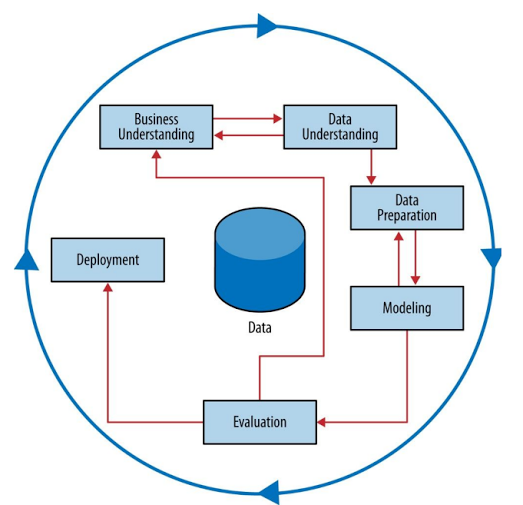
\includegraphics[width=\textwidth]{crisp-dm}
  \caption{Fases do CRISP-DM}
  \label{fig:crispdm}
\end{figure}

O \textbf{Entendimento do negócio} é a primeira etapa e trata-se de conhecer o
problema o qual se quer resolver. Deve-se determinar os objetivos do negócio,
os objetivos da mineração de dados, os critérios de avaliação de sucesso, as
limitações, os riscos e contigências, os custos e benefícios e os recursos
disponíveis. Nesta etapa é produzido um plano do projeto e uma avaliação inicial
de ferramentas e técnicas necessárias.

O \textbf{Entendimento dos dados} consiste na avaliação dos \textit{dados crus}
a partir dos quais será feita a análise. É importante que seja bem compreendido
o potencial e as limitações dos dados disponíveis e se serão necessários
esforços para coleta de novos dados. Esta etapa pode ser entendida em subfases,
consistindo em \textit{Coleta inicial dos dados}, \textit{Descrição dos dados},
\textit{Exploração dos dados} e \textit{Verificação da qualidade dos dados}.

Estas duas primeiras etapas são bastante iterativas entre si, implicando que
um melhor entendimento de cada uma delas pode levar a um aperfeiçoamento da
outra. Dessa forma, é comum que várias iterações sejam feitas entre elas antes
de se passar para a próxima etapa.

A \textbf{Preparação dos dados} consiste em converter os dados disponíveis para
os formatos esperados pelas ferramentas de processamento e análise que serão
utilizadas. Tarefas comuns desta etapa incluem limpeza dos dados (tratamento de
\textit{outliers} e valores faltantes), conversão de tipos de dados, seleção de
dados, identificação de atributos derivados, integração de diferentes conjuntos
de dados e formatação dos dados.

Na fase de \textbf{Modelagem} são aplicadas as técnicas de mineração de dados
para geração de modelos e identificação de padrões nos dados. Comumente, durante
esta etapa é necessário voltar na fase de preparação dos dados para adequar os
dados disponíveis para os formatos esperados.

Na etapa de \textbf{Avaliação} os modelos e padrões extraídos na etapa anterior
são avaliados de acordo com os objetivos do negócio, definidos na primeira fase.
A partir desta etapa é possível ter uma ideia geral de todo o processo e os
resultados alcançados e, sendo necessário, é o momento de realizar uma nova
iteração do ciclo, voltando à etapa de entendimento do negócio. Neste ponto é
possível também determinar os próximos passos, ou seja, as possívei ações e
decisões que podem decorrer do processo.

A fase de \textbf{Implantação} consiste em colocar em uso os modelos gerados
na mineração de dados. Deve ser elaborado um plano de implantação, que muitas
vezes inclui otimizações e adequações dos modelos para o ambiente de produção.
É necessário também que já se planeje como será feito o monitoramento da solução
em produção, assim como sua manutenção. Por fim, pode ser salutar que o projeto
como um todo seja revisto e as experiências acumuladas sejam documentadas.

\subsection{SEMMA}

O acrônimo para \textit{Sample, Explore, Modify, Model, Assess - SEMMA} define
um processo para desenvolvimento de projetos de mineração de dados criado pelo
\href{https://www.sas.com}{SAS Institute} (uma tradicional empresa
desenvolvedora de soluções de \textit{software} analíticos e estatísticos). As
cinco etapas definidas pelo padrão são as seguintes
\cite{wikipedia-semma-2021,azevedo2008}:

A primeira etapa, de \textbf{Amostragem}, consiste em selecionar o conjunto de
dados a ser modelado. O conjunto precisa ser grande o suficiente para conter
informações relevantes a serem extraídas, porém pequeno o suficiente para ser
usado de forma eficiente. Esta etapa também cuida do particionamento dos dados.
De acordo com \citeonline{azevedo2008}, esta etapa é opcional.

A etapa seguinte, de \textbf{Exploração}, cuida do entendimento dos dados,
olhando para a relações entre as variáveis e buscando tendências e anomalias,
com ajuda de mecanismos de visualização de dados.

A etapa de \textbf{Modificação} prepara os dados para modelagem através de
métodos de seleção, criação e transformação de variáveis.

A \textbf{Modelagem} aplica técnicas de mineração de dados para criação de
modelos que que combinem os dados para levar aos resultados desejados.

Por fim, a fase de \textbf{Avaliação} compara os resultados dos modelos de forma
a mensurar a confiabilidade, utilidade e performance dos mesmos.


% ----------------------------------------------------------
% Detalhamento das Metodologias
% ----------------------------------------------------------
\section{Principais diferenças}
\label{sec:diferencas}

Primeiramente vale ressaltar que as três metodologias possuem objetivos
semelhantes e, dessa forma, possuem diversos elementos em comum entre elas. De
uma certa maneira, todas elas implementam subdivisões em três principais blocos
de tarefas bem definidos: \textit{Preparação}, \textit{Modelagem} e
\textit{Avaliação}.

Mais do que um método bem definido, \textit{KDD} é um conjunto de conceitos
que, juntos, levam a uma extração de conhecimento a partir de dados. Não existe
uma especificação oficial e formal de suas etapas, sendo suas práticas
apresentadas de formas ligeiramente diferentes por cada autor.

Já \textit{CRISP-DM} é sim uma metodologia bem definida, com especificação
documentada formalmente, padronização de etapas e nomenclatura. Conta a seu
favor também o fato de ser um padrão aberto, adotado pela União Europeia
\cite{wikipedia-crisp-2021}, e com participação de diversas companhias. Outra
vantagem do modelo é uma melhor especificação dos seus caminhos de iteração,
que ajudam a visualizar quais ciclos podem ser traçados em cada etapa do
projeto. Esta esquemática não é especificada pelos outros dois modelos.

Por sua vez, \textit{SEMMA} também é uma especificação melhor definida, mas tem
a particularidade de ser criada por uma só empresa que, de certa forma, adequa
suas especificações às particularidades das ferramentas produzidas por ela
própria.

Podemos dizer que \textit{CRISP-DM} é mais ampla que as outras metodologias por
especificar as etapas de \textit{Entendimento do negócio} e \textit{Implantação}
(apesar de que na \textit{KDD}, a etapa final de
\textit{Apresentação dos resultados} possa, em alguns aspectos, se assemelhar a
esta etapa de implantação da \textit{CRISP-DM}). Podemos dizer que as etapas da
\textit{SEMMA} seriam mais ``técnicas'' (focadas na mineração de dados), por não
considerarem essas etapas de início e fim que estariam mais ligadas ao
gerenciamento de projeto.

% ---
% Finaliza a parte no bookmark do PDF, para que se inicie o bookmark na raiz
% ---
\bookmarksetup{startatroot}%
% ---

% ---
% Conclusão
% ---
\section{Considerações finais}
\label{sec:final}

As metodologias apresentadas se propõem a objetivos específicos, porém possuem
suas particularidades que tornam uma ou outra mais adequada para determinadas
situações.

\textit{KDD} se aplica como um conjunto mais geral de técnicas e boas práticas,
sendo ideal para cientistas de dados experientes, que conhecem bem as etapas
de mineração de dados e necessitem de um \textit{framework} flexível e modular
que possa se adequar a necessidade de cada projeto em particular.

\textit{CRISP-DM} é um conjunto bem especificado e mais rígido de regras e etapas,
aplicáveis por cientistas novatos ou experientes para qualquer tamanho ou
complexidade de projeto. É o \textit{framework} mais completo, detalhado e
robusto mas, por isso mesmo, as vezes mais complexo do que as necessidades
específicas de um projeto.

\textit{SEMMA} é um \textit{framework} bem especificado e também bastante
adequado para cientistas pouco experientes. É mais focado nas etapas técnicas
do processo e, por isso, mais adequado para projetos que já tenham uma boa
especificação de negócio e ambiente bem definido de homologação e produção.
Apesar de servir para uso geral, se aplica melhor se combinado com a utilização
das ferramentas da mesma empresa que o desenvolveu.

De uma forma geral, se eu fosse inicar um projeto de Ciência de Dados hoje,
tenderia a utilizar o \textit{CRISP-DM}, principalmente pela minha pouca
experiência em projetos desse tipo. Nesta situação, um \textit{framework} mais
robusto e detalhado poderia ser um melhor guia para organização das tarefas.

% ----------------------------------------------------------
% ELEMENTOS PÓS-TEXTUAIS
% ----------------------------------------------------------
\postextual

% ----------------------------------------------------------
% Referências bibliográficas
% ----------------------------------------------------------
\bibliography{20210515-D1INT-atividade02}

\end{document}
